\section{Espaços Métricos Completos}

\subsection{Sequências de Cauchy e Espaços Completos}

\dfn{Sequência de Cauchy}{$(x_n)\subset X$ é de Cauchy quando $\forall\,\eps>0\ \exists\, N(\eps)\in\bbN$
tal que $n,m\geq N \implies d(x_n,x_m)<\eps$.}

\dfn{Espaço Completo, Banach e Hilbert}{$(X,d)$ é completo quando toda sequência de Cauchy converge em
$X$. Um espaço normado $(E,\|\cdot\|)$ é dito completo quando o espaço métrico induzido pela norma é
completo; nesse caso $(E,\|\cdot\|)$ é um \textbf{espaço de Banach}. Um espaço de produto interno
$(E,\langle\cdot,\cdot\rangle)$ é dito completo se o espaço normado induzido pelo produto interno é
completo; nesse caso $(E,\langle\cdot,\cdot\rangle)$ é um \textbf{espaço de Hilbert}.}

\qslista{27}{Sejam $(x_n)$ e $(y_n)$ sequências de Cauchy em um espaço métrico. Mostre que
a sequência $(d(x_n,y_n))$ é convergente.}

\qslista{28}{Se $(x_n)$ é uma sequência de Cauchy que possui subsequência convergente,
mostre que $(x_n)$ converge para o mesmo limite.}

\qslista{29}{Encontre uma métrica $d$ em $\bbR$ de forma que $(\bbR,d)$ não seja completo.}

\qslista{30}{Seja $(X,d)$ um espaço métrico.
\begin{enumerate}
	\item Mostre que $\tilde d(x,y)=\dfrac{d(x,y)}{1+d(x,y)}$ é outra métrica em $X$.
	\item Mostre que $X$ é limitado na métrica $\tilde d$.
	\item Mostre que, se $(X,d)$ é completo, então $(X,\tilde d)$ é completo. Vale a recíproca?
	      Justifique.
\end{enumerate}}

\qslista{31}{Mostre que $(\bbZ,d)$ é completo, sendo $d(m,n)=|m-n|$. De forma geral, mostre
que todo espaço métrico uniformemente discreto é completo.}

\qslista{34}{Mostre que $(X,d)$ é completo se, e somente se, vale a seguinte propriedade:
para toda sequência de bolas fechadas encaixadas $\overline{B}_{j+1}\subset \overline{B}_j$ com raios
$r_j\to 0$, a interseção $\bigcap_{j=1}^{\infty}\overline{B}_j$ consiste de exatamente um ponto.}

\subsection{Completude de $C[a,b]$}

\ex{$C[a,b]$ é completo com a métrica do sup}{$C[a,b]=\{x:[a,b]\to\bbR \mid x \text{ contínua}\}$ é
completo em relação a $d(x,y)=\sup_{t\in[a,b]}|x(t)-y(t)|$.}
\begin{myproof}
	Seja $(x_n)\subset C[a,b]$ sequência de Cauchy. Logo, $\forall t_0\in[a,b]\ \forall\eps>0\ \exists
	N(t_0,\eps)\in\bbN$ tal que
	$$\forall n,m\geq N,\quad |x_m(t_0)-x_n(t_0)|\leq \sup_{t\in[a,b]}|x_m(t)-x_n(t)|<\frac{\eps}{2}\text{.}$$
	Portanto a sequência $(y_k)\subset\bbR$ definida por $y_k=x_k(t_0)$ é de Cauchy e, com isso, existe
	$y_{t_0}\in\bbR$ tal que $y_k\xrightarrow{k\to\infty}y_{t_0}$. Com isso é possível definir
	$$x:[a,b]\to\bbR\text{,}\qquad t\mapsto y_t\text{.}$$
	Note que $x\in C[a,b]$, pois $\forall t_0\in[a,b]$, como $y_k\xrightarrow{k\to\infty}x(t_0)$, existe
	$N_0$ tal que $\ell\geq N_0 \implies |y_\ell-x(t_0)|<\eps$.

	\nt{Verificar que a convergência $x_n\to x$ é, de fato, uniforme em $[a,b]$.}
\end{myproof}

\ex{$C[a,b]$ não é completo com a métrica $L^1$}{Considerando $d(x,y)=\int_a^b |x(t)-y(t)|\,dt$, $C[a,b]$
não é completo. De fato, considere $C[0,1]$.}
\begin{myproof}
	Para cada $m\in\bbN$, seja $x_m:[0,1]\to\bbR$ a função linear por partes que vale $0$ em $[0,a_m]$,
	sobe linearmente até $1$ em $a_m=1-\frac{1}{2m}$, e vale $1$ em $[a_m,1]$:
	\begin{center}
		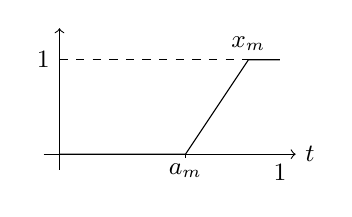
\begin{tikzpicture}[scale=1]
			\draw[->] (-0.2,0) -- (3,0) node[right] {\small $t$};
			\draw[->] (0,-0.2) -- (0,1.6);
			\draw (0,0) -- (1.6,0) -- (2.4,1.2) -- (2.8,1.2);
			\draw[dashed] (0,1.2) -- (2.4,1.2);
			\draw[dashed] (1.6,0) -- (1.6,-0.05);
			\draw (0,1.2) node[left] {\small $1$};
			\draw (1.6,0) node[below] {\small $a_m$};
			\draw (2.8,0) node[below] {\small $1$};
			\draw (2.4,1.4) node {\small $x_m$};
		\end{tikzpicture}
	\end{center}
	Suponha, sem perda de generalidade, que $n>m$. Como $a_n-a_m=\frac{1}{2m}-\frac{1}{2n}$, segue que
	$$d(x_n,x_m)=\frac14\left(\frac1m-\frac1n\right)<\eps\text{,}$$
	logo $(x_m)$ é de Cauchy em relação à métrica $L^1$. Entretanto $(x_m)$ converge, em relação a essa
	métrica, para
	$$x(t)=\begin{cases}0\text{,} & t\in[0,1)\text{,} \\ 1\text{,} & t=1\text{,}\end{cases}$$
	que não é contínua e, portanto, não pertence a $C[0,1]$.
\end{myproof}

\qslista{35}{Sejam $X$ o conjunto das funções $f:[0,1]\to\bbR$ contínuas e
$d(x,y)=\int_0^1|x(t)-y(t)|\,dt$. Mostre que $(X,d)$ não é completo.}
\nt{Cf. exemplo anterior, já demonstrado.}

\qslista{36}{Seja $Y=\{x\in C[a,b] \mid x(a)=x(b)\}\subset C[a,b]$. Mostre que $Y$ é
completo.}

\qslista{47}{Mostre que $C[a,b]$ não é completo em relação à norma $\|x\|_1=\int_a^b
|x(t)|\,dt$. Mostre também que existe $C>0$ tal que $\|x\|_1\leq C\|x\|_\infty$, $\forall x\in C[a,b]$,
sendo $\|\cdot\|_\infty$ a norma usual de $C[a,b]$. Pode existir $C>0$ tal que $\|x\|_\infty\leq
C\|x\|_1$, $\forall x\in C[a,b]$?}

\qslista{48}{Mostre que $C^1[a,b]=\{f:[a,b]\to\bbR \mid f \text{ é continuamente
diferenciável}\}$ é um espaço de Banach com a norma
$$\|x\|=\max_{t\in[a,b]}|x(t)|+\max_{t\in[a,b]}|x'(t)|\text{.}$$}

\subsection{Completude de $\ell^p$}

\mprop{$\ell^p$ é completo, $1\leq p<\infty$}{}
\begin{myproof}
	Seja $(x_n)\subset\ell^p$ de Cauchy, $x_n=\big(x_1^{(n)},x_2^{(n)},x_3^{(n)},\dots\big)$. Então
	$\forall\eps>0\ \exists N(\eps)\in\bbN$ tal que
	$$n,m\geq N \implies d(x_n,x_m)=\sum_{k\in\bbN}\big|x_k^{(n)}-x_k^{(m)}\big|^p<\eps^p\text{.}$$
	Note que, para cada $k\in\bbN$, $\big|x_k^{(n)}-x_k^{(m)}\big|^p\leq d(x_n,x_m)<\eps^p$, logo
	$\big(x_k^{(n)}\big)_{n\in\bbN}$ é de Cauchy em $\bbR$, i.e.,
	\begin{align}
		x_k^{(n)}\xrightarrow{n\to\infty}x_{(k)}\text{.}
	\end{align}
	Com isso definimos $x=\big(x_{(k)}\big)_{k\in\bbN}$ e notamos que $x_n\xrightarrow{n\to\infty}x$.
	Verifiquemos que $x\in\ell^p$:
	$$\sum_{k\in\bbN}\big|x_{(k)}\big|^p=\sum_{k\in\bbN}\Big|\big(x_{(k)}-x_k^{(n)}\big)-\big(-x_k^{(n)}\big)\Big|^p$$
	$$\implies \|x\|_{\ell^p}=d(x-x_n,x_n)\leq d(x,x_n)+\|x_n\|_{\ell^p}\text{,}\quad \forall n\in\bbN\text{.}$$
	Como $x_n\xrightarrow{n\to\infty}x$, dado $\eps_0>0$ existe $N_0\in\bbN$ tal que
	$\|x\|_{\ell^p}<\eps_0+\|x_{N_0}\|_{\ell^p}<+\infty$, pois $(x_n)\subset\ell^p$. Ou seja, sequências de
	Cauchy em $\ell^p$ convergem em $\ell^p$.
\end{myproof}

\subsection{Subespaços Fechados de Espaços Completos}

\nt{Requisitos para o Teorema do Ponto Fixo de Banach.}

\thm{}{Considere $(X,d)$ espaço métrico completo e $F\subset X$. $F$ é fechado $\iff$ $F$ é completo em
relação à métrica induzida de $X$.}
\begin{myproof}
	($\Rightarrow$) Seja $(x_n)\subset F$ sequência de Cauchy. Em particular $(x_n)$ é Cauchy em $X$.
	Assim, $x_n\xrightarrow{n\to\infty}x\in X$. Mas $F$ é fechado e, por consequência, $x\in F$. Logo $F$
	é completo.

	($\Leftarrow$) Suponha $F$ completo. Considere $x\in\bar F$. Logo existe $(x_n)\subset F$ tal que
	$x_n\xrightarrow{(X,d)}x$ e, por consequência, $(x_n)$ é de Cauchy em $F$. Como $F$ é completo, segue
	que existe $y\in F$ tal que $x_n\xrightarrow{(X,d)}y$. Da unicidade do limite em espaços métricos,
	segue que $x=y \implies \bar F=F \implies F$ é fechado.
\end{myproof}

\qslista{32}{Seja $c_{00}\subset\ell^\infty$ o subespaço de todas as sequências com no
máximo uma quantidade finita de termos não nulos. Mostre que $c_{00}$ não é completo em relação à métrica
induzida de $\ell^\infty$.}

\qslista{33}{Sejam $c$ e $c_0$ os subespaços de $\ell^\infty$ formados, respectivamente,
por todas as sequências convergentes e por todas as sequências convergentes para zero. Mostre que $c$ e
$c_0$ são fechados em $\ell^\infty$, logo são completos. Mostre também que esses subespaços são
separáveis.}

\qslista{45}{Sejam $Y$ e $Z$ subespaços de um espaço de Banach $X$. Suponha que existe
$C>0$ tal que
$$\text{dist}(x,Y\cap Z)\leq C\,\text{dist}(x,Y)\text{,}\quad \forall x\in X\text{,}$$
mostre que $Y+Z$ é fechado.}
